\newcommand{\chapter}[2][]{
	\newcommand{\chapname}{#2}
	\begin{flushleft}
		\begin{minipage}[t]{\linewidth}
			
\includegraphics[height=1cm]{hdht-logo.png}
			\hspace{0pt}	
			\sffamily\bfseries\large Bài  33.
			\begin{flushleft}
				\huge\bfseries #1
			\end{flushleft}
		\end{minipage}
	\end{flushleft}
	\vspace{1cm}
	\normalfont\normalsize
}
\chapter[Biến dạng của vật rắn]{Biến dạng của vật rắn}
\section{Lý thuyết}
\subsection{Biến dạng kéo và biến dạng nén}
Khi không có ngoại lực tác dụng, vật rắn có kích thước và hình dạng xác định. Khi có ngoại lực tác dụng, vật rắn thay đổi hình dạng và kích thước, ta nói vật rắn bị biến dạng.

\begin{minipage}{0.4\textwidth}
\subsubsection{Biến dạng kéo}
Dấu hiện nhận biết: Kích thước của vật theo phương tác dụng của lực tăng lên so với kích thước tự nhiên của nó.
\subsubsection{Biến dạng nén}
Dấu hiện nhận biết: Kích thước của vật theo phương tác dụng của lực giảm xuống so với kích thước tự nhiên của nó.
\end{minipage}
\begin{minipage}{0.4\textwidth}
	\begin{center}
		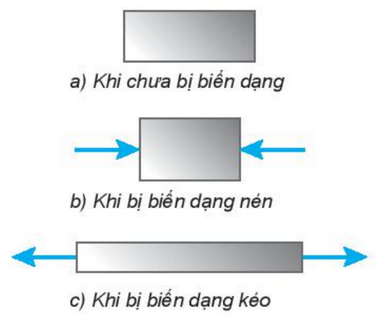
\includegraphics[scale=1]{../figs/G10-028-1}
	\end{center}
\end{minipage}

\section{Mục tiêu bài học - Ví dụ minh họa}
\begin{dang}{Nhận biết đặc điểm của \\ chuyển động tròn đều}
	\viduii{1}{Chuyển động nào dưới đây là chuyển động tròn đều?
		\begin{mcq}
			\item Chuyển động của mắt xích xe đạp khi xe chạy.
			\item Chuyển động của đầu cánh quạt trần khi quay ổn định.
			\item Chuyển động của đầu cánh quạt trần khi vừa bật.
			\item Chuyển động của con lắc đồng hồ.
		\end{mcq}
	}
	{	\begin{center}
			\textbf{Hướng dẫn giải}
		\end{center}
		
		Chuyển động tròn đều là chuyển động có các đặc điểm:
		
		- Quỹ đạo là một đường tròn;
		
		- Tốc độ trung bình trên mọi cung tròn là như nhau.
		
		\textbf{Đáp án: B}.
		
	}
	\viduii{1}{Chuyển động của vật nào dưới đây là chuyển động tròn đều?
		\begin{mcq}
			\item Chuyển động của đầu van bánh xe đạp khi xe đang chuyển động thẳng chậm dần đều.
			\item Chuyển động quay của Trái Đất quanh Mặt Trời.
			\item Chuyển động của điểm đầu cánh quạt trần khi đang quay ổn định.
			\item Chuyển động của điểm đầu cánh quạt khi vừa tắt điện.
		\end{mcq}
	}
	{	\begin{center}
			\textbf{Hướng dẫn giải}
		\end{center}
		
		Chuyển động quay của Trái Đất quanh Mặt Trời là chuyển động tròn đều.
		
		\textbf{Đáp án: B}.
	}
	
\end{dang}
\begin{dang}{Biểu diễn đơn vị độ dịch chuyển góc}
	\viduii{2}{Đổi các góc sau từ độ sang radian: $30^\circ$, $90^\circ$.
	}
	{	\begin{center}
			\textbf{Hướng dẫn giải}
		\end{center}
		
		Ta có:
		$$x^\circ \longrightarrow \dfrac{x \pi}{180}\ \text{rad}.$$
		
		Đổi $$30^\circ \longrightarrow \dfrac{30\pi}{180}\ \text{rad} = \dfrac{\pi}{6}\ \text{rad}$$
		
		Đổi $$90^\circ \longrightarrow \dfrac{90\pi}{180}\ \text{rad} = \dfrac{\pi}{2}\ \text{rad}$$
		
		\begin{center}
			\textbf{Câu hỏi tương tự}
		\end{center}
		
		Đổi các góc sau từ độ sang radian: $105^\circ$, $120^\circ$, $270^\circ$.
		
		\textbf{Đáp án:} $105^\circ \longrightarrow \dfrac{7\pi}{12}\ \text{rad}$; $120^\circ \longrightarrow \dfrac{2\pi}{3}\ \text{rad}$; $270^\circ \longrightarrow \dfrac{3\pi}{22}\ \text{rad}$.
	}
	\viduii{2}{Đổi các góc sau từ radian sang độ: $\SI{0.25}{rad}$, $\SI{0.5}{rad}$.
	}
	{	\begin{center}
			\textbf{Hướng dẫn giải}
		\end{center}
		
		Ta có:
		$$x\ \text{rad} \longrightarrow \dfrac{x \cdot 180}{\pi}\ ^\circ.$$
		
		Đổi $$\SI{0.25}{rad} \longrightarrow \dfrac{0,25 \cdot 180}{\pi} = 14,33^\circ$$
		
		Đổi $$\SI{0.5}{rad} \longrightarrow \dfrac{0,5 \cdot 180}{\pi} = 28,66^\circ$$
		
		\begin{center}
			\textbf{Câu hỏi tương tự}
		\end{center}
		
		Đổi các góc sau từ radian sang độ: $\xsi{0,5\pi}{rad}$, $\xsi{\pi}{rad}$.
		
		\textbf{Đáp án:} $\xsi{0,5\pi}{rad} \longrightarrow 90^\circ$; $\xsi{\pi}{rad} \longrightarrow 180^\circ$.
	}
\end{dang}
\begin{dang}{Tính tốc độ dài, tốc độ góc, chu kỳ, tần số trong chuyển động tròn đều}
	\viduii{2}{Một vệ tinh nhân tạo ở độ cao $250\ \text{km}$ bay quanh Trái Đất theo một quỹ đạo tròn. Chu kì của vệ tinh là $88\ \text{phút}$. Tính tốc độ góc của vệ tinh. Cho bán kính Trái Đất là $6400\ \text{km}$
	}
	{	\begin{center}
			\textbf{Hướng dẫn giải}
		\end{center}
		Khoảng cách từ vệ tinh đến tâm Trái Đất: 
		$$r=250\ \text{km}+6400\ \text{km} =6650\ \text{km}=6650000\ \text{m}. $$
		Tốc độ góc của vệ tinh:
		$$T=\frac{2\pi}{\omega} \Rightarrow \omega = \frac{\pi}{2640}\ \text{rad/s}.$$ 
		
		\begin{center}
			\textbf{Câu hỏi tương tự}
		\end{center}
		
		Roto trong một tổ máy của nhà máy thủy điện Hòa Bình quay 125 vòng mỗi phút. Hãy tính tốc độ góc của roto này theo đơn vị rad/s.
		
		\textbf{Đáp án:} $\omega \approx \SI{13.1}{rad/s}$.
	}
	
	\viduii{3}{
		Kim phút của đồng hồ dài gấp 1,5 lần kim giờ. Hỏi tốc độ dài của đầu kim phút lớn gấp mấy lần tốc độ dài của đầu kim giờ?
	}
	{	\begin{center}
			\textbf{Hướng dẫn giải}
		\end{center}
		
		Gọi $\omega_1, \omega_2$ lần lượt là tốc độ góc của kim phút và kim giờ. Kim phút quay một vòng ($2\pi\ \SI{}{\radian}$) trong 1 giờ ($\SI{3600}{\second}$), kim giờ quay một vòng trong 12 giờ, do đó 
		$$
		\dfrac{\omega_1}{\omega_2}=12
		$$
		
		Ta lập được tỉ số: $$\dfrac{v_1}{v_2}=\dfrac{\omega_1 \cdot R_1}{\omega_2 \cdot R_2}=\dfrac{\omega_1}{\omega_2}\cdot\dfrac{R_1}{R_2}=18.$$
		
		\begin{center}
			\textbf{Câu hỏi tương tự}
		\end{center}
		
		Biết chiều dài kim phút và kim giây của một chiếc đồng hồ lần lượt là $\SI{4}{cm}$ và $\SI{5}{cm}$. Hãy tính:
		\begin{enumerate}[label=\alph*)]
			\item Tỉ số chu kì quay của hai kim.
			\item Tỉ số tốc độ của đầu kim phút và đầu kim giây.
		\end{enumerate}
		
		\textbf{Đáp án:}
		\begin{enumerate}[label=\alph*)]
			\item $\frac{T_\text{phút}}{T_\text{giây}}=60$.
			\item $\frac{v_\text{phút}}{v_\text{giây}}=\dfrac{1}{75}$.
		\end{enumerate}
	}
	
	
	
\end{dang}